\documentclass[a4paper]{article}

\usepackage[UTF8]{ctex}
\usepackage[a4paper,margin=1in]{geometry}
\usepackage{graphicx}
\usepackage{float}
\usepackage{listings}
\usepackage{longtable}
\usepackage{booktabs}
\usepackage{hyperref}
\usepackage{fancyhdr}
\usepackage{lastpage}
\usepackage{color}
\usepackage{indentfirst}        % 首段缩进
\setlength{\parindent}{2em}     % 缩进2字符
\usepackage{zhnumber}           % 中文编号
\usepackage[dvipsnames]{xcolor}

%\newcommand{\college}{中山大学计算机学院}
\newcommand{\projname}{数据库系统原理实验| 实验三}
\newcommand{\reporttitle}{熟悉使用select语句进行数据库的查询}
\newcommand{\stuno}{23336179}
\newcommand{\authorname}{马福泉}
\newcommand{\major}{计算机科学与技术}
\newcommand{\adviser}{赖韩江}
\newcommand{\startdate}{2025年10月9日}
\newcommand{\labenddate}{2025年10月9日}
\newcommand{\labroom}{B202}

\pagestyle{fancy} % 使用 fancyhdr 风格
\fancyhf{}      % 清空默认的页眉页脚

% 设置页眉
\fancyhead[L]{\kaishu \projname}      % 左侧页眉显示项目名称
\fancyhead[C]{\kaishu \reporttitle}    % 中间页眉显示报告标题
\fancyhead[R]{\kaishu \authorname} % 右侧页眉显示作者姓名

% 设置页脚
\fancyfoot[C]{第 \thepage 页，共 \pageref{LastPage} 页} % 中间页脚显示页码

% 去除页眉页脚与正文之间的分隔线
\renewcommand{\headrulewidth}{0.4pt}
\renewcommand{\footrulewidth}{0pt}

% 设置文档背景颜色
\definecolor{mybgcolor}{RGB}{0, 0, 0} % 定义背景颜色
\definecolor{NavyBlue}{RGB}{0,0,128} % 添加颜色定义
% \pagecolor{mybgcolor} % 设置背景颜色

% listing 配置rust
% \lstdefinelanguage{Rust}{
%   keywords={fn, let, mut, struct, enum, impl, pub, use, mod, trait, where},
%   keywordstyle=\color{NavyBlue},
%   comment=[l]{//},
%   commentstyle=\color{gray},
% }
% \lstset{language=Rust}

\lstset{
  basicstyle=\ttfamily\small,
  keywordstyle=\color{NavyBlue},
  commentstyle=\color{gray},
  stringstyle=\color{red},
  showstringspaces=false,
  extendedchars=false, % 关键：不处理中文
  breaklines=true
}

\begin{document}

% 封面
\begin{titlepage}
    \centering
    

    
\includegraphics[width=10cm]{img/SYSULogo.png}

    \vspace{1em}
    %{\Large \college \par}
    \vspace{1em}
    {\Large \kaishu \projname \par}
    \vspace{3em}

    

    
    {\fontsize{40pt}{42pt}\kaishu \selectfont \boldmath \reporttitle\par}
    \vspace*{\fill}

    \begin{center}
    {\Large
    \makebox[5em][s]{学号}:\underline{\makebox[15em][c]{\kaishu \stuno}}\\[1em]
    \makebox[5em][s]{姓名}:\underline{\makebox[15em][c]{\kaishu \authorname}}\\[1em]
    \makebox[5em][s]{专业}:\underline{\makebox[15em][c]{\kaishu \major}}\\[1em]
    \makebox[5em][s]{课程教师}:\underline{\makebox[15em][c]{\kaishu \adviser}}\\[1em]
    \makebox[5em][s]{起始日期}:\underline{\makebox[15em][c]{\kaishu \startdate}}\\[1em]
    \makebox[5em][s]{结束日期}:\underline{\makebox[15em][c]{\kaishu \labenddate}}\\[1em]
    \makebox[5em][s]{实验地点}:\underline{\makebox[15em][c]{\kaishu \labroom}}
    }
    \end{center}

    \vspace*{\fill}
\end{titlepage}

% 目录
\tableofcontents
\newpage


\section{实验概述}

\subsection{实验目的}

熟悉使用select语句进行数据库的查询。

\subsection{实验内容}

在实验二修改后的数据库基础上（如下表），使用SELECT子句设定查询内容，要求附上执行结果（数据库）截图。

\begin{table}[H]
\centering
\caption{图书表}
\label{tab:books}
\begin{tabular}{|p{1.2cm}|p{2.5cm}|p{2.5cm}|p{2.5cm}|p{2.5cm}|p{2.5cm}|p{2.5cm}|}
\hline
\textbf{book\_id} & \textbf{book\_name} & \textbf{book\_isbn} & \textbf{book\_author} & \textbf{book\_publisher} & \textbf{book\_price}& \textbf{interviews\_times}  \\
\hline
b0001 & SQL Server 2012宝典 & 978-7-121-22013-5 & 廖梦怡 & 电子工业出版社 & 18.00 & 10 \\
\hline
b0002 & 职称英语专用教材 & 978-7-121-14800-2 & 孙若红 & 电子工业出版社 & 35.00 & 10 \\
\hline
b0003 & 中国通史 & 978-7-5388-53155 & 于海娣 & 黑龙江科学技术出版社 & 25.00 & 0 \\
\hline
b0004 & 丰子恺儿童文学选集 & 978-7-5007-8972-7 & 丰子恺 & 中国少年儿童出版社 & 40.00 & 0 \\
\hline
b0005 & 英语同义词辨析词典 & 978-7-5135-2294-6 & 赵同水 & 外语教学与研究出版社 & 6.00 & 0 \\
\hline
b0006 & 数据库基础与应用 & 978-7-304-06430-3 & 徐孝凯 & 中央广播电视大学出版社 & 5.00 & 0 \\
\hline
b0007 & 微积分初步 & 978-7-304-03742-0 & 赵坚 & 中央广播电视大学出版社 & 4.00 & 0 \\
\hline
b0008 & ASP.NET从入门到精通 & 978-7-302-28753-7 & 明日科技 & 清华大学出版社 & 27.00 & 0 \\
\hline
\end{tabular}
\end{table}

\begin{table}[H]
\centering
\caption{读者表}
\label{tab:readers}
\begin{tabular}{|c|c|c|c|}
\hline
\textbf{reader\_id} & \textbf{reader\_name} & \textbf{reader\_sex} & \textbf{reader\_department} \\
\hline
r0001 & 李德海 & 男 & 信息工程系 \\
\hline
r0002 & 柳承运 & 男 & 信息工程系 \\
\hline
r0004 & 谢嫣然 & 女 & 涉外教育系 \\
\hline
r0005 & 陈静玉 & 女 & 涉外教育系 \\
\hline
r0006 & 李媛媛 & 女 & 经济管理系 \\
\hline
r0007 & 胡锦波 & 男 & 经济管理系 \\
\hline
r0008 & 蔡明伟 & 男 & 行政管理系 \\
\hline
\end{tabular}
\end{table}

\begin{table}[H]
\centering
\caption{借阅记录表}
\label{tab:record}
\begin{tabular}{|c|c|c|c|c|}
\hline
\textbf{reader\_id} & \textbf{book\_id} & \textbf{borrow\_date} & \textbf{return\_date} & \textbf{notes} \\
\hline
r0001 & b0003 & 2014-01-12 & 2014-01-12 & NULL \\
\hline
r0001 & b0005 & 2014-01-26 & 2014-06-21 & NULL \\
\hline
r0004 & b0001 & 2014-03-02 & 2014-04-20 & NULL \\
\hline
r0004 & b0008 & 2014-03-26 & 2014-05-28 & NULL \\
\hline
r0006 & b0001 & 2014-04-16 & 2014-07-11 & NULL \\
\hline
r0007 & b0006 & 2014-05-08 & 2014-09-17 & NULL \\
\hline
\end{tabular}
\end{table}

\begin{table}[H]
\centering
\caption{借阅统计表}
\label{tab:borrow_statistics}
\begin{tabular}{|c|c|}
\hline
\textbf{reader\_id} & \textbf{borrow\_count} \\
\hline
r0001 & 2 \\
\hline
r0004 & 2 \\
\hline
r0006 & 1 \\
\hline
r0007 & 1 \\
\hline
r0008 & 2 \\
\hline
\end{tabular}
\end{table}

\begin{table}[H]
\centering
\caption{读者表2}
\label{tab:reader2}
\begin{tabular}{|c|c|c|c|}
\hline
\textbf{reader\_id} & \textbf{reader\_name} & \textbf{reader\_sex} & \textbf{reader\_department} \\
\hline
r0003 & 安歌 & 女 & 涉外教育系 \\
\hline
r0004 & 谢嫣然 & 女 & 涉外教育系 \\
\hline
r0005 & 陈静玉 & 女 & 涉外教育系 \\
\hline
\end{tabular}
\end{table}

具体实验内容：\\
1. 查询图书表book的所有信息\\
2. 查询读者表reader的读者姓名和所在院系\\
3. 查询读者表reader的读者姓名和所在系，要求查询结果显示为"姓名"和"院系"\\
4. 查询图书表book的所有信息，只显示查询结果的前5行数据\\
5. 查询图书表book的出版社名称，要求出版社名称不重复显示\\
6. 查询数据表book的借阅次数的总和，要求查询结果显示为"总借阅次数"\\
7. 在读者表reader中统计读者总人数\\
8. 查询读者表reader中所有姓"王"的读者的信息\\
9. 查询图书表book中所有图书信息，并按借阅次数由高到低进行排序\\
10. 在图书表book中统计各出版社出版图书的总数\\
11. 在图书表book中查询图书借阅次数在20次以上，而且出版图书总数大于1的出版社\\
12. 查询没有借阅编号为"b0005"这本书的读者姓名\\
13. 查询借阅至少2本书的读者姓名\\
14. 查询借阅次数最多和最少的图书编号（要求使用=any）\\
15. 查询借阅过图书编号为"b0002"图书的读者编号和姓名\\
16. 查询编号为"r0007"读者的姓名、所在院系以及所借阅图书的书名\\
17. 查询没有借阅过图书，以及借阅图书次数最多的读者信息，要求查询结果显示为"姓名"，"性别"和"院系"

\section{实验报告}

\subsection{实验步骤与结果}

\subsubsection{查询1：查询图书表book的所有信息}

\begin{lstlisting}[language=SQL, caption=查询图书表所有信息]
SELECT * FROM book;
\end{lstlisting}

\begin{figure}[H]
\centering
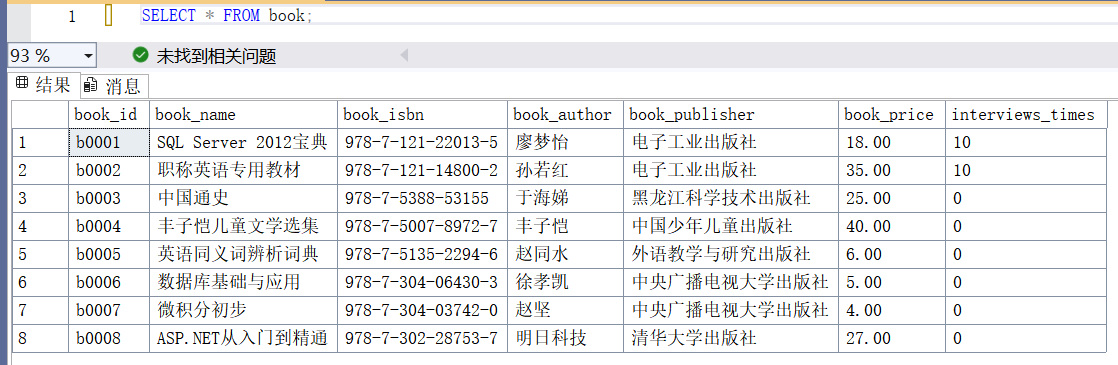
\includegraphics[width=0.8\textwidth]{img/query1_result.png}
\caption{查询图书表所有信息结果}
\label{fig:query1}
\end{figure}

\subsubsection{查询2：查询读者表reader的读者姓名和所在院系}

\begin{lstlisting}[language=SQL, caption=查询读者姓名和所在院系]
SELECT reader_name, reader_department FROM reader;
\end{lstlisting}

\begin{figure}[H]
\centering
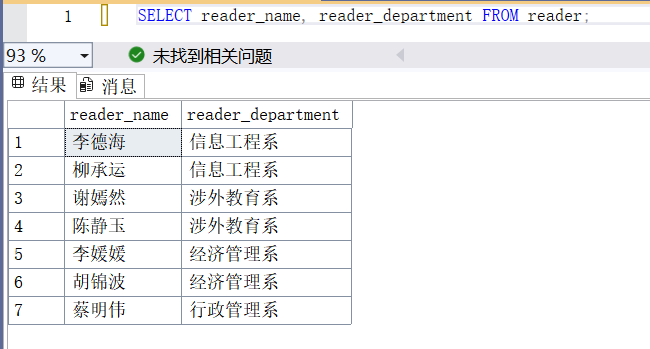
\includegraphics[width=0.8\textwidth]{img/query2_result.png}
\caption{查询读者姓名和所在院系结果}
\label{fig:query2}
\end{figure}

\subsubsection{查询3：查询读者表reader的读者姓名和所在系，要求查询结果显示为"姓名"和"院系"}

\begin{lstlisting}[language=SQL, caption=查询读者姓名和所在系并重命名列]
SELECT reader_name AS '姓名', reader_department AS '院系' FROM reader;
\end{lstlisting}

\begin{figure}[H]
\centering
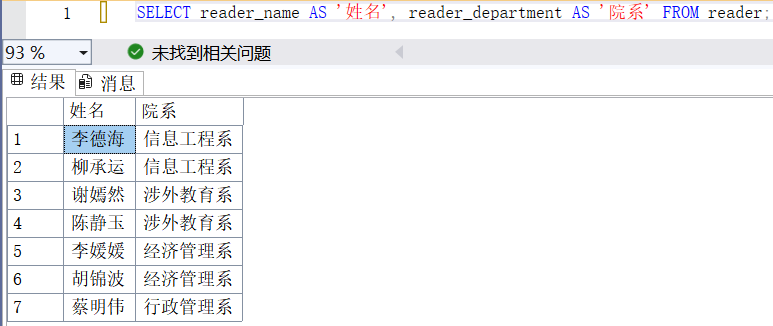
\includegraphics[width=0.8\textwidth]{img/query3_result.png}
\caption{查询读者姓名和所在系并重命名列结果}
\label{fig:query3}
\end{figure}

\subsubsection{查询4：查询图书表book的所有信息，只显示查询结果的前5行数据}

\begin{lstlisting}[language=SQL, caption=查询图书表前5行数据]
SELECT TOP 5 * FROM book;
\end{lstlisting}

\begin{figure}[H]
\centering
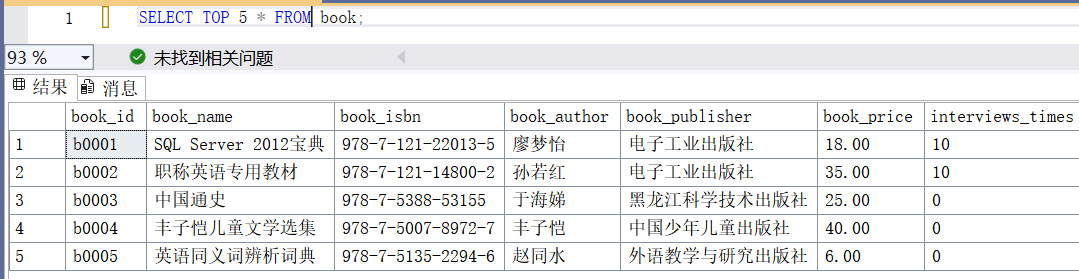
\includegraphics[width=0.8\textwidth]{img/query4_result.png}
\caption{查询图书表前5行数据结果}
\label{fig:query4}
\end{figure}

\subsubsection{查询5：查询图书表book的出版社名称，要求出版社名称不重复显示}

\begin{lstlisting}[language=SQL, caption=查询不重复的出版社名称]
SELECT DISTINCT book_publisher FROM book;
\end{lstlisting}

\begin{figure}[H]
\centering
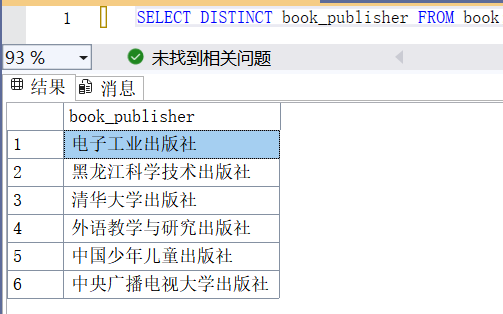
\includegraphics[width=0.8\textwidth]{img/query5_result.png}
\caption{查询不重复的出版社名称结果}
\label{fig:query5}
\end{figure}

\subsubsection{查询6：查询数据表book的借阅次数的总和，要求查询结果显示为"总借阅次数"}

\begin{lstlisting}[language=SQL, caption=查询借阅次数总和]
SELECT SUM(interviews_times) AS '总借阅次数' FROM book;
\end{lstlisting}

\begin{figure}[H]
\centering
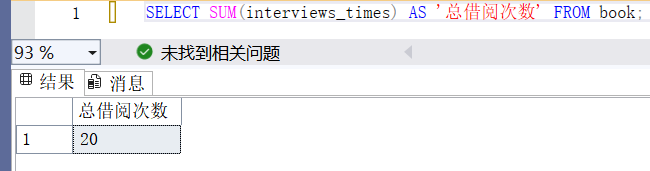
\includegraphics[width=0.8\textwidth]{img/query6_result.png}
\caption{查询借阅次数总和结果}
\label{fig:query6}
\end{figure}

\subsubsection{查询7：在读者表reader中统计读者总人数}

\begin{lstlisting}[language=SQL, caption=统计读者总人数]
SELECT COUNT(*) AS '读者总人数' FROM reader;
\end{lstlisting}

\begin{figure}[H]
\centering
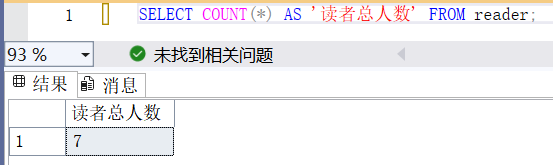
\includegraphics[width=0.8\textwidth]{img/query7_result.png}
\caption{统计读者总人数结果}
\label{fig:query7}
\end{figure}

\subsubsection{查询8：查询读者表reader中所有姓"王"的读者的信息}

\begin{lstlisting}[language=SQL, caption=查询所有姓王的读者信息]
SELECT * FROM reader WHERE reader_name LIKE '王%';
\end{lstlisting}

\begin{figure}[H]
\centering
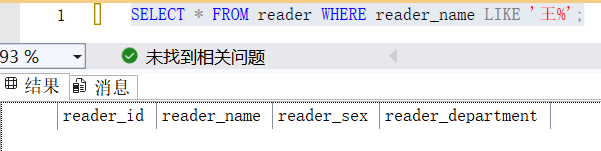
\includegraphics[width=0.8\textwidth]{img/query8_result.png}
\caption{查询所有姓王的读者信息结果}
\label{fig:query8}
\end{figure}

\subsubsection{查询9：查询图书表book中所有图书信息，并按借阅次数由高到低进行排序}

\begin{lstlisting}[language=SQL, caption=按借阅次数降序查询图书信息]
SELECT * FROM book ORDER BY interviews_times DESC;
\end{lstlisting}

\begin{figure}[H]
\centering
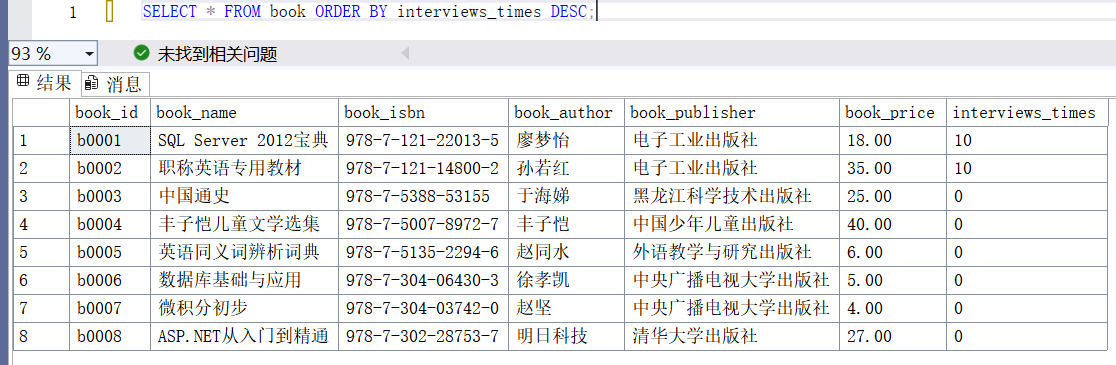
\includegraphics[width=0.8\textwidth]{img/query9_result.png}
\caption{按借阅次数降序查询图书信息结果}
\label{fig:query9}
\end{figure}

\subsubsection{查询10：在图书表book中统计各出版社出版图书的总数}

\begin{lstlisting}[language=SQL, caption=统计各出版社出版图书总数]
SELECT book_publisher AS '出版社', COUNT(*) AS '图书总数' 
FROM book 
GROUP BY book_publisher;
\end{lstlisting}

\begin{figure}[H]
\centering
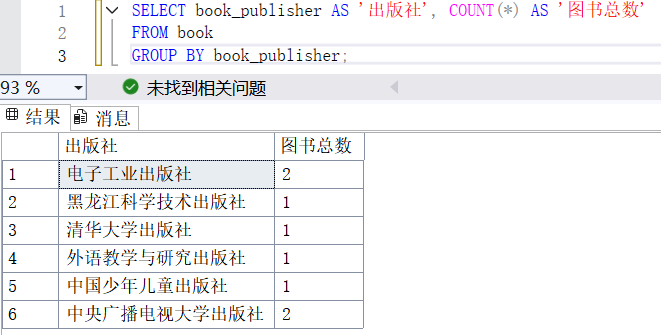
\includegraphics[width=0.8\textwidth]{img/query10_result.png}
\caption{统计各出版社出版图书总数结果}
\label{fig:query10}
\end{figure}

\subsubsection{查询11：在图书表book中查询图书借阅次数在20次以上，而且出版图书总数大于1的出版社}

\begin{lstlisting}[language=SQL, caption=查询符合条件的出版社]
SELECT book_publisher AS '出版社', COUNT(*) AS '图书总数'
FROM book 
GROUP BY book_publisher
HAVING SUM(interviews_times) >= 20 AND COUNT(*) > 1;
\end{lstlisting}

\begin{figure}[H]
\centering
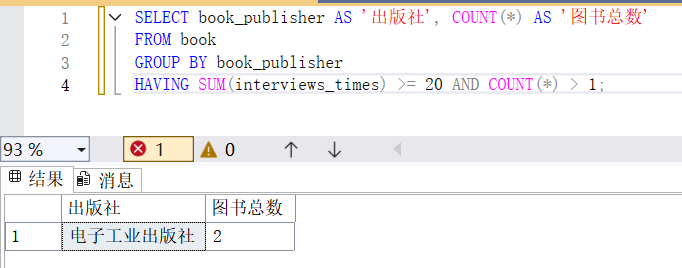
\includegraphics[width=0.8\textwidth]{img/query11_result.png}
\caption{查询符合条件的出版社结果}
\label{fig:query11}
\end{figure}

\subsubsection{查询12：查询没有借阅编号为"b0005"这本书的读者姓名}

\begin{lstlisting}[language=SQL, caption=查询没有借阅指定图书的读者]
SELECT reader_name 
FROM reader 
WHERE reader_id NOT IN (
    SELECT reader_id 
    FROM record 
    WHERE book_id = 'b0005'
);
\end{lstlisting}

\begin{figure}[H]
\centering
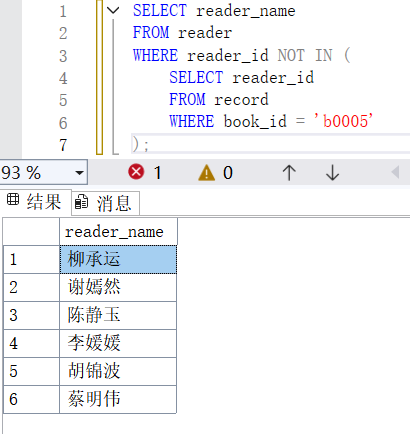
\includegraphics[width=0.8\textwidth]{img/query12_result.png}
\caption{查询没有借阅指定图书的读者结果}
\label{fig:query12}
\end{figure}

\subsubsection{查询13：查询借阅至少2本书的读者姓名}

\begin{lstlisting}[language=SQL, caption=查询借阅至少2本书的读者]
SELECT r.reader_name 
FROM reader r
INNER JOIN (
    SELECT reader_id 
    FROM record 
    GROUP BY reader_id 
    HAVING COUNT(*) >= 2
) rec ON r.reader_id = rec.reader_id;
\end{lstlisting}

\begin{figure}[H]
\centering
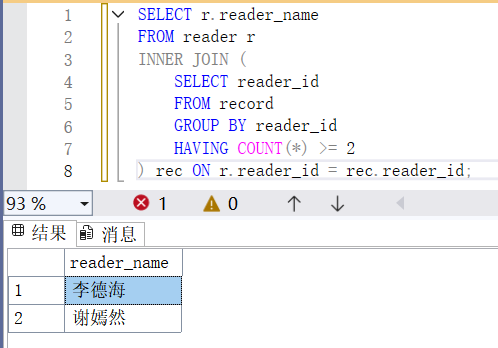
\includegraphics[width=0.8\textwidth]{img/query13_result.png}
\caption{查询借阅至少2本书的读者结果}
\label{fig:query13}
\end{figure}

\subsubsection{查询14：查询借阅次数最多和最少的图书编号（要求使用=any）}

\begin{lstlisting}[language=SQL, caption=查询借阅次数最多和最少的图书编号]
SELECT book_id, interviews_times 
FROM book 
WHERE interviews_times = ANY (
    SELECT MAX(interviews_times) FROM book
    UNION 
    SELECT MIN(interviews_times) FROM book
);
\end{lstlisting}

\begin{figure}[H]
\centering
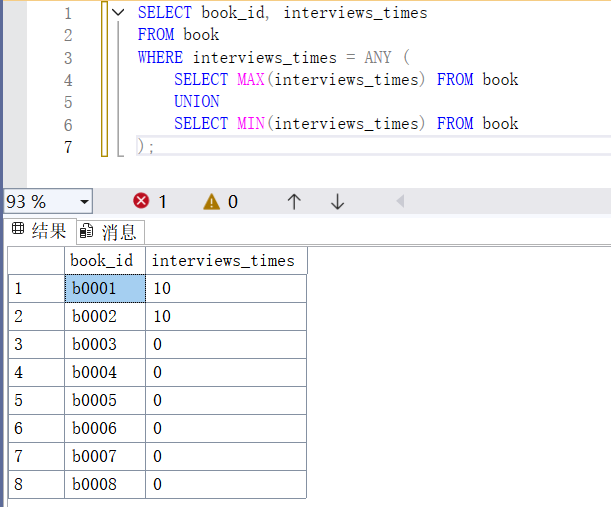
\includegraphics[width=0.8\textwidth]{img/query14_result.png}
\caption{查询借阅次数最多和最少的图书编号结果}
\label{fig:query14}
\end{figure}

\subsubsection{查询15：查询借阅过图书编号为"b0002"图书的读者编号和姓名}

\begin{lstlisting}[language=SQL, caption=查询借阅指定图书的读者信息]
SELECT DISTINCT r.reader_id, r.reader_name 
FROM reader r
INNER JOIN record rec ON r.reader_id = rec.reader_id
WHERE rec.book_id = 'b0002';
\end{lstlisting}

\begin{figure}[H]
\centering
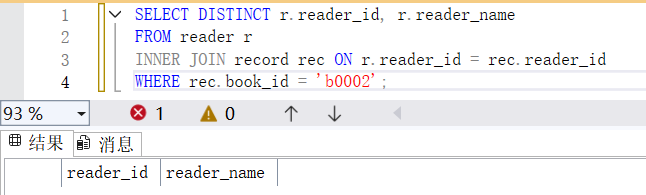
\includegraphics[width=0.8\textwidth]{img/query15_result.png}
\caption{查询借阅指定图书的读者信息结果}
\label{fig:query15}
\end{figure}

\subsubsection{查询16：查询编号为"r0007"读者的姓名、所在院系以及所借阅图书的书名}

\begin{lstlisting}[language=SQL, caption=查询指定读者的详细借阅信息]
SELECT r.reader_name, r.reader_department, b.book_name
FROM reader r
INNER JOIN record rec ON r.reader_id = rec.reader_id
INNER JOIN book b ON rec.book_id = b.book_id
WHERE r.reader_id = 'r0007';
\end{lstlisting}

\begin{figure}[H]
\centering
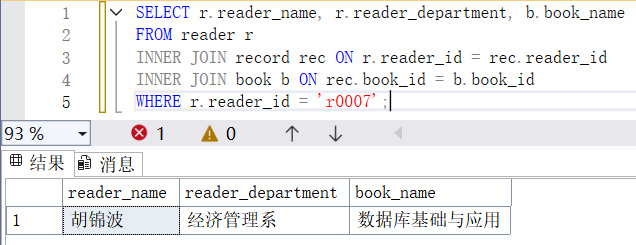
\includegraphics[width=0.8\textwidth]{img/query16_result.png}
\caption{查询指定读者的详细借阅信息结果}
\label{fig:query16}
\end{figure}

\subsubsection{查询17：查询没有借阅过图书，以及借阅图书次数最多的读者信息，要求查询结果显示为"姓名"，"性别"和"院系"}

\begin{lstlisting}[language=SQL, caption=查询没有借阅过图书和借阅次数最多的读者]
-- 查询没有借阅过图书的读者
SELECT reader_name AS '姓名', reader_sex AS '性别', reader_department AS '院系'
FROM reader 
WHERE reader_id NOT IN (SELECT DISTINCT reader_id FROM record)

UNION

-- 查询借阅次数最多的读者
SELECT r.reader_name AS '姓名', r.reader_sex AS '性别', r.reader_department AS '院系'
FROM reader r
INNER JOIN (
    SELECT reader_id, COUNT(*) as borrow_count
    FROM record 
    GROUP BY reader_id
    HAVING COUNT(*) = (
        SELECT MAX(borrow_count) 
        FROM (
            SELECT COUNT(*) as borrow_count 
            FROM record 
            GROUP BY reader_id
        ) t
    )
) max_borrow ON r.reader_id = max_borrow.reader_id;
\end{lstlisting}

\begin{figure}[H]
\centering
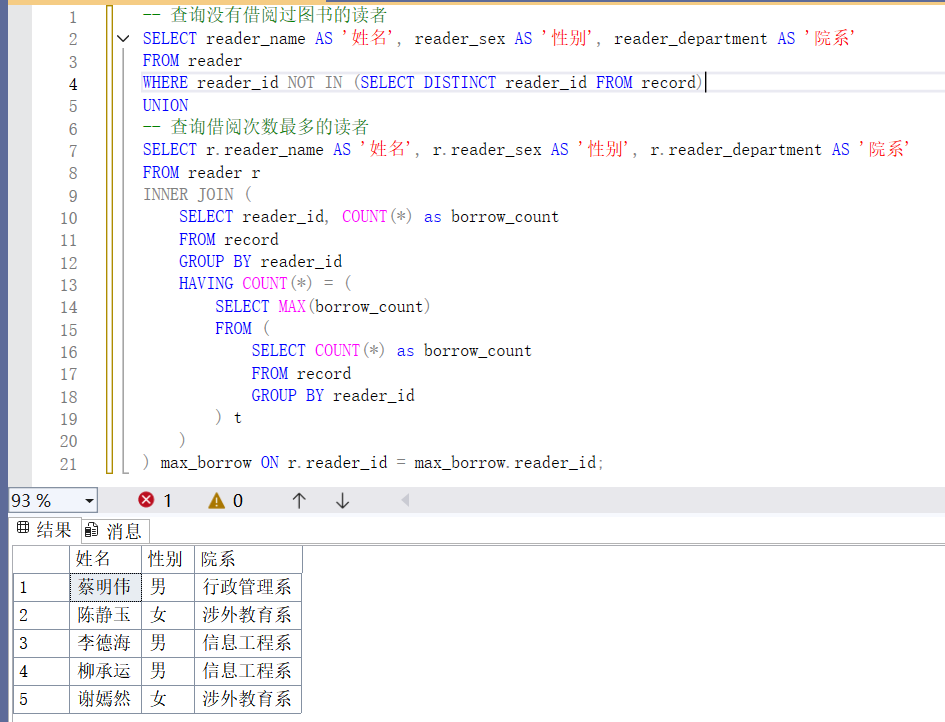
\includegraphics[width=0.8\textwidth]{img/query17_result.png}
\caption{查询没有借阅过图书和借阅次数最多的读者结果}
\label{fig:query17}
\end{figure}

\subsection{实验总结}

通过本次实验，我全面掌握了SQL SELECT语句的各种用法：

\begin{enumerate}
    \item \textbf{基础查询}：学会了使用SELECT语句进行简单的数据查询，包括全表查询和指定列查询。
    \item \textbf{列别名}：掌握了使用AS关键字为查询结果的列设置别名，提高查询结果的可读性。
    \item \textbf{数据限制}：学会了使用TOP关键字限制查询结果的行数。
    \item \textbf{去重查询}：熟练运用DISTINCT关键字去除查询结果中的重复数据。
    \item \textbf{聚合函数}：掌握了SUM、COUNT、MAX、MIN等聚合函数的使用方法。
    \item \textbf{条件查询}：学会了使用WHERE子句进行条件筛选，包括LIKE模糊查询、比较运算符等。
    \item \textbf{排序}：熟练运用ORDER BY子句对查询结果进行排序。
    \item \textbf{分组查询}：掌握了GROUP BY和HAVING子句的使用，能够进行分组统计查询。
    \item \textbf{子查询}：学会了在WHERE、HAVING等子句中使用子查询，包括IN、NOT IN、ANY等操作符。
    \item \textbf{连接查询}：掌握了INNER JOIN等连接操作，能够查询多表关联数据。
    \item \textbf{联合查询}：学会了使用UNION操作符将多个查询结果合并。
\end{enumerate}

本次实验大大提升了我对SQL查询语句的理解和运用能力，为后续的数据库开发工作奠定了坚实的基础。

\textbf{易错点分析：}
\begin{itemize}
    \item \textbf{字段名拼写错误或表名错误}，会导致SQL语句执行失败。
    \item \textbf{子查询返回多行时用=而不是IN}，会报错或结果不正确。
    \item \textbf{连接查询时未指定连接条件}结果数量异常。
    \item \textbf{使用TOP、LIMIT等关键字时注意数据库类型}，不同数据库语法可能会略有差异。
    \item \textbf{模糊查询LIKE语法}
    \item \textbf{UNION合并查询时字段数量和类型需一致}。
\end{itemize}

\end{document}